\chapter{Design}
\label{sec:design}

% Ist das zentrale Kapitel der Arbeit. Hier werden das Ziel sowie die
% eigenen Ideen, Wertungen, Entwurfsentscheidungen vorgebracht. Es kann
% sich lohnen, verschiedene Möglichkeiten durchzuspielen und dann
% explizit zu begründen, warum man sich für eine bestimmte entschieden
% hat. Dieses Kapitel sollte - zumindest in Stichworten - schon bei den
% ersten Festlegungen eines Entwurfs skizziert werden.
% Es wird sich aber in einer normal verlaufenden
% Arbeit dauernd etwas daran ändern. Das Kapitel darf nicht zu
% detailliert werden, sonst langweilt sich der Leser. Es ist sehr
% wichtig, das richtige Abstraktionsniveau zu finden. Beim Verfassen
% sollte man auf die Wiederverwendbarkeit des Textes achten.

% Plant man eine Veröffentlichung aus der Arbeit zu machen, können von
% diesem Kapitel Teile genommen werden. Das Kapitel wird in der Regel
% wohl mindestens 8 Seiten haben, mehr als 20 können ein Hinweis darauf
% sein, daß das Abstraktionsniveau verfehlt wurde.

% Die Lösung kurz vorstellen. also du hast dich für die lösung mit dem dc network entschieden und das wurde bisher noch nicht vorgeschlagen in der wissenschaft. Dann sagen bevor du das prinzip vorstellt werden erstmal alle Teilnehmer, die in dem System vorkommen, vorgestellt. dazu auch das bild aus der technischen richtlinie benutzen, wo smartmeter und smart meter admin. welche netzwerke also han etc...
%Dann sagen, dass du erstmal auf das angreifermodell eingehst und dann dc netz erklären und dann die lösung vorschlagen.
%die lösung wurde noch nicht diskutiert, weil in der wissenschaft immer davon ausgegangen wurde, dass smart meter nicht sicher sind,wir gehen davon aus, dass ein smart meter vertraut werden kann und das man deshalb auch nicht auf das billing eingehen muss, weil das smart meter korrekt arbeitet und das billing deshalb trivial ist. der stromanbieter kann auch prüfen  bzw. die logeinträge sind fälschungssicher.

This chapter outlines the conceptual solution of this thesis to achieve privacy-preserving smart meters. The proposed protocol can be categorized as aggregation without a trusted third party. Before discussing the conceptual solution, the technical guideline from the BSI will be explained. The BSI is the cyber-security authority of the German government and is responsible for critical infrastructures such as smart grids in Germany.  The technical guideline TR-03109 resolves all security standards and security concepts that must be met by all power grid providers in Germany. Therefore, the technical guideline gives a good overview of the actual structure of the German power grid. After getting an overview of the power grid and its participants, an attacker model will be designed. The attacker model will introduce all necessary participants, what their motives are and what malicious motives they might pursue. Finally, the security protocol will be presented. It will be shown how the protocol can be integrated into the technical policy and how different potentially malicious participants are handled.

\section{Technical guideline TR-03109}
This paragraph will discuss the technical guideline published by the BSI (Federal Office for Information Security). The BSI is the entity of the German federal government that deals with digital security issues and issues recommendations as well as mandatory security guidelines for critical infrastructures. Among other things, technical guidelines are published in which security standards are defined for different IT systems. The technical guideline BSI-TR-03109 defines minimum requirements for the functionality, security and interoperability of smart meters in Germany.  The technical guideline BSI-TR-03109 defines minimum requirements for functionality, security and interoperability that individual components of smart meters in Germany must fulfill. The guideline as a whole consists of 6 different documents, which are shown in Figure 3.1. Based on the guidelines, it is possible to have devices certified by test centers. Unless otherwise described, all information are derived from the technical guideline.\\
\\
\textbf{Actors on the SMGW}
%hier ein kleiner text
\\
\\
\begin{enumerate}
\item Consumer: \\
The consumer is the person who uses electrical energy, gas, water
or heat. In addition, the consumer is the owner of the measurements processed and stored in the SMGW. In order to interact with the SMGW, the consumer uses a communication device. All necessary data can be retrieved and displayed through it.\\
\item SMGW administrator:\\
A Smart Meter Gateway Administrator (GWA) a trusted entity and each SMGW is assigned a GWA. The GWA handles the configuration, monitoring and control of SMGWs and it is even possible to perform updates of SMGWs via the GWA.\\
\item Authorized external entities:\\
External market participants (EMT) are all other authorized participants in the energy network that can establish a communication connection with the SMGW.These include power grid providers and electricity suppliers. The SMGW ignores all other communication requests that do not come from the GWA or EMTs in order to prevent attacks.\\
\end{enumerate}
There are several other actors such as Controllable Local Systems, service technicians and meters. However, these actors do not play a major role in the protocol that is proposed here.
\begin{figure}[tbp]
  \centering
  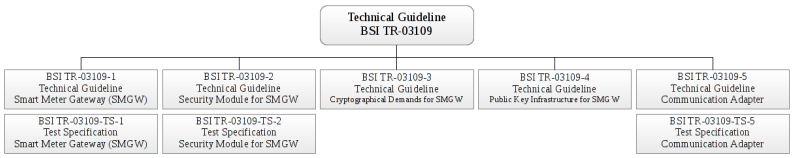
\includegraphics[width=1\textwidth]{images/BSI-TR-03109.png}
  \caption[Short description]{An example of a NILM analysis.}
  \label{fig:Appliance_Model}
\end{figure}
\\
\\
\textbf{Interfaces and functions of the Smart Meter Gateway}
\\
\\
A smart meter or as described in the technical guideline a smart meter gateway(SMGW) must provide 3 different physical interfaces.
\begin{enumerate}
\item Local Metrological Network (LMN):\\
The LMN is the communication interface in which communication takes place with the connected meters for energy and material quantities (electricity, gas). An SMGW can communicate with one meter from one end user or with several meters from different end users. In practice, however, one SMGW is often responsible for one meter. The measured values are sent from the meters via the LMN to the SMGW and stored there.
\item Wide Area Network (WAN):\\
The WAN is the only communication interface with which the SMGW can communicate with EMTs or GWAs over the Internet. If a request is made to the SMGW that was not sent by these authorized participants, then the request is discarded and ignored.
\item Home Area Network (HAN):\\
In HAN, an SMGW interacts with Controllable Local Systems (e.g., photovoltaic systems). In addition, users and service technicians can use the HAN interface to display information about power consumption through functions offered by the SMGW.
\end{enumerate}
\begin{figure}[tbp]
  \centering
  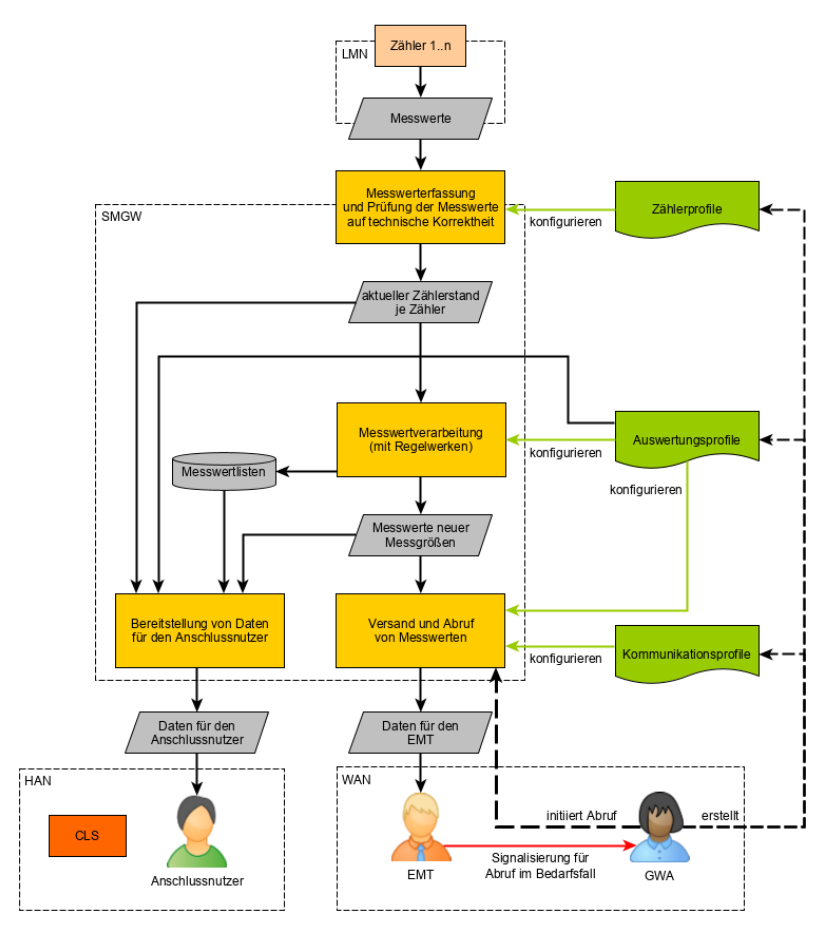
\includegraphics[width=1\textwidth]{images/Messwertverarbeitung.png}
  \caption[Short description]{An example of a NILM analysis.}
  \label{fig:Appliance_Model}
\end{figure}
\textbf{Functionality of the smart meter gateway}
\\
\\
First, the task of SMGW is to store the measurements sent by meters from the LMN. Then, the readings are processed in the SMGW and sent to the authorized EMTs in the WAN after processing. An SMGW must also perform the tasks of a firewall and separate the 3 interfaces. It is therefore impossible for an EMT or GWA to make requests to devices located in the HAN or LMN, even if it is allowed to interact with the SMGW over the WAN.
Since the WAN interface is the most important interface for this work, it will be discussed in more detail.\\
\\
\textbf{Functions of the SMGW in the WAN}
\\
\\
The tasks performed by the WAN have already been explained in the paragraph above. Now the functions and security mechanisms offered by the SMGW to guarantee secure interaction on the WAN will be described.
\begin{enumerate}
\item Transmission of measured values based on evaluation and WAN communication profiles:\\
Communication profiles of GWAs are stored in SMGW. The communication profiles determine how the data is processed in the SMGW and forwarded to EMTs.

\item Pseudonymization:\\
Data that is not relevant for billing must be pseudonomized for data protection reasons. For this purpose, the unique identification number that each SMGW has is replaced by a pseudonym. Subsequently, the information is not sent directly to an EMT, but is forwarded to the EMT via the GWA. This additionally protects the identity of the sending SMGW.%vllt als extra part machen. was unten kommt.
Even if peusodonymization does not allow an SMGW to be directly assigned, the described attack in [ref] and the resulting behavioral analysis is still possible. Since no other security mechanisms are available from the SMGW, the question must be asked whether pseudonymization as proposed in the technical guideline is sufficient.

\item Time synchronization:\\
In order for the cost electricity consumption to be calculated correctly, it is essential that the SMGW have an accurate time. For this purpose, the system time of the SMGW is synchronized with the time server of the GWA at regular intervals.

\item Wake-Up Service:\\
A GWA is able to force a communication link with the SMGW. This is done via a data packet signed by the GWA. The SMGW then establishes a fixed preconfigured communication connection to the GWA. This enables the GWA to execute administration commands on the SGMW. 
\end{enumerate}
\section{Adversary Model}
It has already been explained in this chapter which participants in the power grid interact with each other. Now in particular it will be discussed which motives the different participants have and which malicious motives can be pursued by the participants or by attackers.  \\
\\
The smart meter attempts to achieve the 3 security objectives of confidentiality, integrity and availability. The 3 security goals are often summarized as CIA. Another important security goal for this work is anonymity. The 4 definitions are essential for the understanding of this work. Therefore, the terms are explained below.
\begin{enumerate}
\item Confidentiality: \\
It is not possible for an unauthorized party to gain information about the content of the data sent.
\item Integrity:\\
It is not possible for an unauthorized party to modify the content of data without data without this being noticed.
\item Availability: \\
It is not possible for an unauthorized party to interfere with the functionality of a service.
\item Anonymity:\\
Verbergen der Identität vor dem Kommunikationspartner???
Vllt wer hat die Daten gesendet, wer hat den Stromverbrauch gesendet?
\end{enumerate}
 
 
All available attacks will aim at bypassing these security targets to get information about the customer. 
\subsection{Customer's Motives}
For the costumer, all the security goals defined above are important. But by far the most important is the security goal of anonymity through the smart meter. Possible attacks on the electricity consumption penetrate deeply into the private sphere of each customer. Therefore, no conclusions may be drawn from the electricity consumption of a customer.\\
On the other hand, unethical customers may try to steal electricity to save energy costs. The smart meter is located in or on the customer's house. An unethical customer could attempt to tamper directly with the smart meter's hardware or software. The attempts could look like this, a Costumer could try to reduce the recorded electricity consumption at the Smart meter or the Smart meter could be manipulated to measure less electricity when electricity prices are high and more electricity when electricity prices are low.
\subsection{Electricity Provider's Motives}
For the electricity provider, the authenticity of the billing is the most important security objective because From the electricity provider's point of view, the customer is not trustworthy in the calculation of the bill. In addition, the customer has access to the smart meter at almost any time in an environment trusted by the customer. Unlike analog meters, smart meters cannot be mechanically attacked. But if a customer manages to change the software of the smart meter, the billing can be manipulated at the same time. On the other hand, the electricity provider can also be an overly intrusive electricity provider. In the paragraph [Ref NILM] it was explained how a behavioral analysis can be created from the electricity consumption. This sensitive information could be used to gain an additional source of income. In [SSRN] it was listed which questions could be answered by a Nilm analysis. Quote: "On what days and during what times do you watch TV? How much home time do you spend in front of your computer?" or "Are any of the appliances in your household failing or operating below optimal efficiency? Do you own (and so presumably like) lots of gadgets?". Advertising companies would certainly pay money for this kind of information in order to be able to advertise more accurately.
\subsection{Eavesdropping}
Eavesdropping may be the weakest type of attack, but successful eavesdropping on the communications of the smart meter could be useful to e.g. intruders. However, curious neighbors might also have an interest in the behavior inside the house. Turning on/off lights implies that someone is at home or leaving the house. Therefore, eavesdropping on electricity consumption could provide information about when is a suitable time to break in. To prevent eavesdropping, smart meter communication is encrypted to maintain confidentiality. Cryptographic algorithms such as AES are widely used today and have been analyzed for weaknesses over the years by a number of researchers. Hence, a successful attack on encrypted data to extract information is extremely unlikely.
\subsection{Active Attackers}
In Germany, the smart grid is one of the critical infrastructures. This means that the failure of the smart grid could lead to a significant compromise of public safety or other serious consequences. Such systems are threatened by active attackers. The objective of active attackers may not necessarily be to analyze a user's electricity consumption. They may want to disable availability through e.g. denial of service attacks. These attacks could leave major damage to the power grid and are definitely a realistic threat [quelle]. But this thesis focuses on smart meters and the anonymization of electricity consumption. That's why it is assumed that the active attacker does not carry out system-wide attacks on the power grid. Rather, it is assumed that the attacker attempts to take control in the proposed DC network. Among other things, it is assumed that the attacker has the theoretical ability to take over one or more SMGW and send messages through the SMGW. In addition, if the attacker has taken over an SMGW, it can perform all operations that are possible through the proposed DC network. In the next section, the conceptual solution of the DC-Net is proposed and how the DC-Net could be implemented in the technical guideline of the BSI. It also describes which attacks on the DC-Net are possible with the defined attacker model.
\section{A Privacy-Preserving Aggregation Scheme Using DC-Nets}
In [Cha3-85, Cha8-85, Chau-88], David Chaum proposes a protocol which he calls DC network. The DC network offers the possibility to achieve both sender anonymity and receiver anonymity in communication networks. The operation of the DC network is explained in the following.
\subsection{DC Networks}
The DC network uses the property that any finite alphabet can be numerated( e.g a=0, b=1 etc). If an numerated alphabet from 0 is given, then this alphabet forms an abelian group (modulo alphabet size). Because of the abelian group, simple mathematical operations like addition can be performed on the numerated letters in the alphabet.
In addition, a DC network assumes that messages are always sent that are of equal length. A participant in a DC network uses one or more keys with which it superposes the messages and one generated key is then communicated to exactly one participant. 
More precisely, each participant adds locally all key characters it generates. Then, the received keys from other participants are locally subtracted and finally, all meaningful characters (the message) that should be sent are added (modulo alphabet size). The result of the operation is distributed in the communication network and is called local superposition. 
The distributed superpositions are added together globally and the result is transmitted back to all participants. Thereby only the meaningful messages remain. If a participant does not want to send a meaningful message, the participant sends an empty message. The message consists only of zeros and is superposed with the key. The empty message reflects the neutral element in this structure. If all participants have sent only empty messages, the global result is a message only containing 0. If one of all participants have sent a meaningful message, the global superposition is the message. If more than one participant sent a meaningful message, then the result is the overlay of all sent messages and a single message from the overlay cannot be recovered. In the last case one speaks also of a collision. In order to solve this problem, the collision resolution algorithm with averaging can be used in a DC network. 
Exchanging keys to calculate the local sum can be very tedious. In addition, a different key must be exchanged for each message round. Otherwise it would be very easy to calculate the key from previously sent empty messages. Therefore, so-called pseudo-random number generators are commonly used. The participants share the initial values of the pseudo-random number generators with each other when they join the DC network. This can be done in the same way as the exchange of keys (e.g. a cryptographic key exchange procedure). Due to the deterministic property of PRNGs, the same sequence of numbers is always generated from an initial value. This in turn means that the initial value must remain secret and must not be revealed to any other participant, since otherwise the secret keys can be found out from the initial value. The consequence would be the loss of anonymity. The security of the DC network depends largely on how secure the PRNGs are. Therefore, the PRNGs that are used must be cryptographically secure.\\
\begin{figure}[tbp]
  \centering
  \includegraphics[scale=1]{images/Schlüsselgraph.png}
  \caption[Short description]{An example of a NILM analysis.}
  \label{fig:Appliance_Model}
\end{figure}
The principle of the DC network is illustrated graphically in figure 3.3 using a simple example. Figure 3.3 is also called the key graph of a DC network and shows 4 participants in a DC network that are connected to each other along a communication link. The outer participants have only one partner, the inner participants are connected to 2 partners. Each participant now exchanges keys with its direct partners. The outer partners need to exchange only one key and the inner ones exchange keys with two direct partners.
The mathematical operation indicates whether the participant adds or subtracts the exchanged key with the partner. In the example given in the figure, the user Petra would subtract the exchanged key with Rüdiger from the message and would have formed her local superposition. Rudiger would have to add the exchanged key with Petra to his message. He would also have to subtract the key he exchanged with Sabine from the result to calculate his local superposition. 

%peusodzufallsgeneratoren
\subsection{DC Network Protocol in a German Smart Grid}
The DC network is a scheme that can be used to achieve sender anonymity and receiver anonymity. Considering the use case of the thesis, the receiver anonymity does not have to be implemented. The aim is to anonymize the electricity consumption and send it to the electricity provider. In this case, the electricity provider is a public recipient and known to all participants. Therefore, the identity of the electricity provider does not need to be protected. Unlike in a normal DC network, the participants do not want to communicate with each other, they only want to send their electricity consumption to the electricity provider. The only exception is when joining the DC network, there the customers have to perform a key exchange once to configure the initial value for the PRNG as explained in 3.3.2.\\
\\
\textbf{Protocol Header}
\\
\\\begin{figure}[tbp]
  \centering
  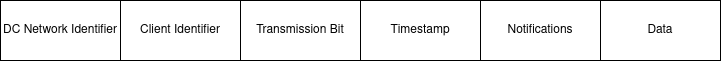
\includegraphics[width=1\textwidth]{images/Header.png}
  \caption[Short description]{An example of a NILM analysis.}
  \label{fig:Appliance_Model}
\end{figure}Each frame in the DC network protocol has the following structure.
As first field there is a Protocol Identifier field. The purpose of the Protocol Identifier field is to ensure that the application of the DC net protocol is recognized by all participants and that the SMGWs as well as the electricity provider can react correctly to the frames. This is followed by the DC Network Identifier field. The DC network identifier field offers the electricity provider the possibility to operate several DC networks in different regions and to distinguish DC networks. In addition, each SMGW is given a unique identifier so that the SMGWs can be distinguished. If the network needs to perform error correction, SMGWs can be notified by the identification number from the power supplier. Although the SMGWs can be identified by the field, the electricity provider still cannot draw any conclusions about electricity consumption from the local superposition. The transmission bit indicates that an SMGW has sent a message and it is used for error correction procedures. The timestamp field indicates when a message was sent. This allows the electricity provider to classify messages by round and not charge for messages from different rounds. The second to last field is the notification field. The field is used for error codes. The electricity provider can thus send notifications to the SMGWs to start error correction procedures. In the last field, the Data field, only the local superpositions are sent.\\
\\
\textbf{Protocol Initialization}
\\
\\
For the Protocol Initialization it is assumed that the electricity provider wants to create a completely new DC network. First, a unique and unchangeable DC Net Identifier is assigned from the electricity provider to the empty DC Net. At least 2 SMGWs have to enter the DC Net. A DC Net with only one participant is not operational and cannot offer anonymity. According to the Technical guideline TR-03109 from BSI, SMGWs are only allowed to communicate with authorized participants in the smart grid and all foreign requests are ignored. These are EMTs, GWAs and the electricity provider. In order for the DC grid to become operational, two SMGW must exchange an initial value to configure the PRNGs. A start value is exchanged once with which both PRNGs of the clients are initialized. As a result, the same random number sequences are generated independently of each other by the PRNG on both clients. But there is a communication barrier that does not allow SMGWs to communicate with other SMGWs. With the limited communication capabilities, the SMGWs rely on the electricity provider. The SMGWs can use a key exchange protocol like Diffie-Helman to transmit the initial value. %Diffie-hellman erklären
Diffie-Hellman is a known key exchange protocol, where 2 users can publicly exchange a secret without a third person being able to figure out the secret.

SMGWs can generate cryptographically secure keys because they have a hardware security module built in. Therefore Key exchange procedures such as Diffie-Hellman can be implemented for the SMGW without any problems. Diffie-Hellman was also only mentioned as an example. There are various attacks on the Diffie-Hellman variant presented.% quelle?
The forwarding of SMGW messages by the electricity provider enables the implementation of other substantially secure key exchange procedures. The advantage of this approach is that SMGWs are anonymous to other SMGWs. When the keys are exchanged, only the partners with whom the key is currently exchanged are aware of it. Uninvolved SMGWs do not receive any information about the entry of new users in a DC network. In addition, the participants share their client identifiers during the key exchange. Due to the exchanged communication details, each participant in the DC network knows the identification number of its neighbor. This is later helpful for error correction measures. %Vllt angriffe nach dem Kapitel SChreiben?
\\The use of a key exchange method also has disadvantages. By forwarding messages, the electricity provider knows which SMGW have exchanged keys with each other. Exchanging keys is equivalent to creating an edge in the key graph.%referenz hinzufügen als ich keygraphs erklärt habe
Therefore, the electricity provider can easily replicate the key graph of the DC network. The knowledge about the structure of the key graph alone does not give the electricity provider any further knowledge, but a malicious electricity provider could use the knowledge to launch active attacks on individual SMGW. An example would be that a electricity provider wants to get information about the power consumption of an SMGW. The electricity provider could connect one or more SMGWs it controls to the victim SMGW through a key exchange that the attacker SMGW launches. The electricity provider could now hope that in the future the victim SMGW will only have keys with the attacker SMGW. Since the electricity provider controls the attacker SMGW and knows the keys of the attacker SMGW, it can reconstruct the electricity consumption of the victim SMGW from the local superposition. \\
\\
\textbf{SGMW Registration in a DC Network}
\\
\\
An SMGW that wants to register in the DC network sends a special defined request to its power provider. For this purpose the notification field in the header is used and notification 1 is sent. Notification 1 represents a request from the SMGW to register in a DC network. The electricity provider assigns the requesting DC client to a suitable geographical region and suggests a suitable client (SMGW) which is already registered in the DC network. The electricity provider now establishes a tunnel and sends the tunnel information to the DC client and the registering client. Via this tunnel it is possible for the two SGMW to establish a communication link via the electricity provider. If an SMGW sends to the tunnel, the message is forwarded to the future neighbor. The DC client which is already present in the DC network is only informed by the electricity provider that it receives a new neighbor and has to exchange contact information. The requesting SMGW needs to send the seeds over the tunnel. To prevent the electricity provider from reading the seeds, the clients exchange Diffie Helmann keys via the tunnels provided.%ist das korrekt?
Once the seeds have been exchanged, the power provider is informed by the requesting client that it has successfully entered the DC network by notification 3. Subsequently, all participants in the DC network can send their local superpositions to the power provider. Here, the number sequences are used as keys, which are generated from the synchronized PRNGs. Subsequently, the local superpositions are sent to the electricity provider. The provider forms the global superposition and receives the aggregated power consumption of all SMGWs in the DC network. The local
The electricity provider is responsible for ensuring that messages can be exchanged between the registered clients via the tunnel already in use, if required. The already registered clients can therefore not choose which new communication partners they get. In addition it is assumed that the electricity provider has already been authorized by the SWA. Otherwise, the SMGW would not be able to establish a connection to the supplier.\\
%(der Gedanke ist, dass es viele verschiedene kleine DC-Netze gibt, die getrennte Schlüsselgraphen besitzen, jedes DC-Netz sendet seine lokale Summe an den Stromanbieter, der alle Werte aufsummiert und die globale Summe bildet (für ein DC-Netz)
\\
\textbf{SGMW Normal Operation}
\\
\\
wie sieht eine normale Operation aus? wie häufig wird gesendet? wofür wird das transmisson bit verwendet? und der timestampt
\\
\\
\textbf{SGMW Exit from the DC Network}
\\
\\
An exit can be caused, for example, when the customer changes the electricity provider. Then a defined message is sent to the electricity provider when an exit occurs. The electricity provider informs the neighbors of the exiting client with a notification message 4. In addition, the DC Client Identifier of the exiting SMGW is sent with the notification message 4. This notification signals to the neighbors of the exiting SMGW that they must discard their PRNG configurations to client X and that they must not be used in the calculation of the local superposition in the next round. In order to avoid a synchronization error in the DC network, the "neighbors" must confirm to the power provider that all seeds have been discarded. Otherwise the case may occur that a SMGW continues to add the old key to its message. This would result in a useless global sum. Furthermore, the key graph must be considered. It could be the case that the underlying key graph splits into two DC networks. If this is the case, two separated DC networks are sending to the same DC network identifier. In the example of Figure 3.3, this could happen if Sabine and Rüdiger throw away their shared key. The result is different depending on the position where a DC net splits. But at least one DC network experiences a significant loss of anonymity due to the smaller number of participants that can be aggregated. In the case of particularly serious splits, it can even lead to a participant being completely disconnected from the DC network. If a disconnected client notices that it no longer has any neighbors, it sends a special emergency message to the power provider. Then a new registration process is initiated before the next round starts.\\ To avoid splitting into two DC networks, the exiting SMGW informs its neighbors with which direct partners it was connected. These then initiate a registration process and exchange keys with each other. The fact that all neighbors have exchanged keys with each other guarantees that a DC network does not split when an SMGW leaves.\\
\\ 
\textbf{SGMW Connection loss}
\\
\\
SMGWs have an Internet connection with which they can communicate in the WAN. If the Internet connection is interrupted, this can lead to an SMGW not being able to send its local superposition in time.
\todo{write design}

\cleardoublepage

%%% Local Variables:
%%% TeX-master: "diplom"
%%% End:
